\documentclass{article}
\usepackage{amsmath}
\usepackage{amssymb}
\usepackage{bm}
\usepackage{graphicx}
\usepackage{epstopdf}
\DeclareGraphicsRule{.tif}{png}{.png}{`convert #1 `basename #1 .tif`.png}
\usepackage{color}
\pagestyle{plain}
%\pagestyle{empty}
\textheight 9 true in
\textwidth 6.5 true in
\hoffset -.75 true in
\voffset -.75 true in
 
\mathsurround=2pt  \parskip=2pt
\def\crv{\cr\noalign{\vskip7pt}} 
\def\a{\alpha } \def\b{\beta } \def\d{\delta } \def\D{\Delta } \def\e{\epsilon }
\def\g{\gamma } \def\G{\Gamma} \def\k{\kappa} \def\l{\lambda } \def\L{\Lambda }
\def\th{\theta } \def\Th{\Theta} \def\r{\rho} \def\o{\omega} \def\O{\Omega}
\def\ve{\varepsilon} 

\def\sA{{\cal A}} \def\sB{{\cal B}} \def\sC{{\cal C}} \def\sI{{\cal I}}
\def\sR{{\cal R}} \def\sF{{\cal F}} \def\sG{{\cal G}} \def\sM{{\cal M}}
\def\sT{{\cal T}} \def\sH{{\cal H}} \def\sD{{\cal D}} \def\sW{{\cal W}}
\def\sL{{\cal L}} \def\sP{{\cal P}} \def\s{\sigma } \def\S{\Sigma}
\def\sU{{\cal U}} \def\sV{{\cal V}} \def\sY{{\cal Y}}

\def\gm{\gamma -1}
\def\summ{\sum_{j=1}^4}

\def\bb{{\bm b}} \def\yb{{\bm y}}
\def\ub{{\bm u}}  \def\xb{{\bm x}} \def\vb{{\bm v}} \def\wb{{\bm w}}
\def\omegab{{\bm \omega}} \def\rb{{\bm r}} \def\ib{{\bm i}} \def\jb{{\bm j}}
\def\lb{{\bm l}} \def\kb{{\bm k}} \def\Ab{{\bm A}} \def\fb{{\bm f}} \def\Ub{{\bm U}}
\def\Fb{{\bm F}} \def\nb{{\bm n}} \def\Db{{\bm D}} \def\eb{{\bm e}}
\def\gb{{\bm g}}  \def\Gb{{\bm G}} \def\hb{{\bm h}} \def\Yb{{\bm Y}} \def\Rb{{\bm R}} 
\def\Tb{{\bm T}}

\def\As1{{\bf {\cal A}}_1}\def\DO{{\cal D}_0} \def\UO{{\cal U}_0}
\def\ie{{\it{i.e.}}}

\def\ubbar{{\bf {\bar{u}}}} \def\sbar{{\bar{\sigma }}} \def\ubar{{\bar{u}}}  
\def\abar{{\bar{a}}} \def\vbar{{\bar{v}}}  \def\rbar{{\bar{\rho}}}
\def\pbar{{\bar{p}}} \def\ebar{{\bar{e}}} \def\Tbar{{\bar{T}}}
\def\bbar{{\bar{\beta}}} \def\Mbar{{\bar{M}}}  \def \sMbar{{\bar{\cal M}}}
\def\Ebar{{\bar{E}}} \def\sMbar{{\bar{\cal M}}}
\def\sPbar{{\bar{\cal P}}} \def\xbar{{\bar{x}}}

\newcommand{\pdv}[2]{\frac{\partial#1}{\partial#2}}
\newcommand{\dv}[2]{\frac{d#1}{d#2}}
\newcommand{\ord}[2]{#1^{(#2)}}
\newcommand{\vct}[1]{\vec{#1}}

 \newcommand{\bc}{\begin{center}}
 \newcommand{\ec}{\end{center}}
 
 \newcommand{\bq}{\begin{equation}}
 \newcommand{\eq}{\end{equation}}
 
 \newcommand{\beqs}{\begin{eqnarray}}
 \newcommand{\eeqs}{\end{eqnarray}}
 
 \newcommand{\beqa}{\begin{eqnarray*}}
 \newcommand{\eeqa}{\end{eqnarray*}}
 
 \newcommand{\ol}{\overline}
 \newcommand{\ul}{\underline}
 
 \newcommand{\dint}{{\int \!\! \int \!\!}}
 \newcommand{\tint}{{\int \!\! \int \!\! \int \!\!}}
 
 \newcommand{\bfig}{\begin{figure}}
 \newcommand{\efig}{\end{figure}}
 
 \newcommand{\cen}{\centering}
 \newcommand{\n}{\noindent}
 
 \newcommand{\btab}{\begin{table}}
 \newcommand{\etab}{\end{table}}
 
 \newcommand{\btbl}{\begin{tabular}}
 \newcommand{\etbl}{\end{tabular}}
 
 \newcommand{\bdes}{\begin{description}}
 \newcommand{\edes}{\end{description}}
 
 \newcommand{\benum}{\begin{enumerate}}
 \newcommand{\eenum}{\end{enumerate}}
 
 \newcommand{\bite}{\begin{itemize}}
 \newcommand{\eite}{\end{itemize}}
 
 \newcommand{\cle}{\clearpage}
 \newcommand{\npg}{\newpage}
 
 \newcommand{\bss}{\begin{singlespace}}
 \newcommand{\ess}{\end{singlespace}}
 
 \newcommand{\bhalf}{\begin{onehalfspace}}
 \newcommand{\ehalf}{\end{onehalfspace}}
 
 \newcommand{\bds}{\begin{doublespace}}
 \newcommand{\eds}{\end{doublespace}}
 
 \newcommand{\eps}{\mbox{$\epsilon$}} 
 \newcommand{\stilde}{\mbox{$\tilde s$}} 
 \newcommand{\shat}{\mbox{$\hat s$}} 

 \newcommand{\blue}{\color{blue}}
 \newcommand{\red}{\color{red}}
 \newcommand{\magenta}{\color{magenta}}
 \newcommand{\green}{\color{green}}
 \newcommand{\nc}{\normalcolor}




%\pagestyle{empty}
\begin{document}

\begin{center}
\large{ MATH-6620 \hspace{1in}  PERTURBATION METHODS \hspace{1in}SPRING 2016\\ Test 1 \\ March 10, 2016}\end{center}


\vspace{6 ex}

{\bf Name: Michael Hennessey} \hfill

\vspace{6 ex}
\textbf{I have abided by the ground rules of this test.}
\vspace {6 ex}

\bc {\bf PROBLEMS} \ec

\benum
\item
\benum
\item Noting that $\tan{x}\to\infty$ as $x\to \pi/2 -$, obtain three terms of a perturbative solution to 
$$\tan{x}=\frac{1}{\e}.$$

\item Find a 3-term asymptotic expansion of the function $x(\e)$ defined by the equation
$$\e e^x=1+\frac{\e}{1+x}.$$
\eenum

Solution:\\

\benum
\item Since we know that the expansion of $x$ is centered about $\pi/2$ as it satisfies
$$\lim_{\e\to 0}\frac{1}{\e}=\tan x,$$
we can attempt a perturbative solution in the form of
$$x=\frac{\pi}{2}+\e x_1+\e^2 x_2+...,$$
but we will quickly see that there is no convenient way to expand $\tan x$ in terms of powers of $\e$. However, we can rewrite the equation in question using the substitution $y=x-\pi/2$ to be able to expand $y$ about $0.$ Thus we have
$$\tan(y+\frac{\pi}{2})=\frac{1}{\e}\implies \e\cos y=-\sin y.$$
Then if we expand each $\cos y$ and $\sin y$ in their respective Taylor series about $y=0$, we get
$$\e\left(1-\frac{y^2}{2}+\frac{y^4}{4!}+...\right)=-\left(y-\frac{y^3}{3!}+\frac{y^5}{5!}+...\right).$$
Then, if we let $y=\e y_1+\e^2 y_2+\e^3$, our equation becomes
$$\e-\frac{\e^3 y_1}{2}-\e^4y_1y_2+...=-\e y_1-\e^2 y_2-\e^3 y_3+\frac{\e^3y_1}{3!}.$$
From here, we look specifically at the powers of $\e$ present.
$$\e^1:\quad 1=-y_1\implies y_1=-1.$$
$$\e^2:\quad 0=-y_2\implies y_2=0.$$
$$\e^3:\quad -\frac{y_1}{2}=-y_3+\frac{y_1}{6}\implies y_3=-\frac{2}{3}.$$
Then since 
$$y=-\e-\e^3\frac{2}{3},$$
we know
$$x=\frac{\pi}{2}-\e-\e^3\frac{2}{3}.$$

\item Plotting each side of the equation with $\e=.01$ shows that we are looking for two expansions of $x(\e).$
\begin{figure}[h]
  \centering
  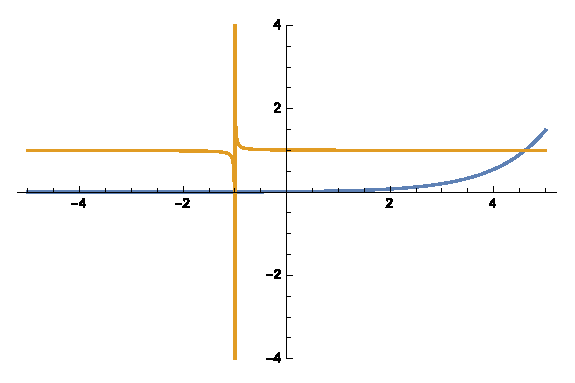
\includegraphics[width=3in]{test1no1prtb}
  \caption{Plot of $.01e^x$ and $1+\frac{.01}{1+x}$.}
\end{figure}
    
    Multiplying each side of the equation in question by $1+x$ and moving the consequent $\e$ term to the left-hand side of the equation results in the equation
    $$\e[(1+x)e^x-1]=1+x.$$
    Now we make successive approximations for $x$. 
    $$1.\quad 0=1+x_0\implies x_0=-1.$$
    $$2.\quad -\e=1+x_1\implies x_1=-1-\e.$$
    $$3.\quad \e[-\e e^{-1-\e}-1]=1+x_2\implies x_2=-1-\e-\e^2 e^{-1-\e}.$$
    Giving the 3-term asymptotic expansion
    $$x_l(\e)=-1-\e-\e^2 e^{-1-\e}.$$
    Clearly this solution is the left solution pictured above, corresponding to the singularity of the equation at $x=-1.$ Thus we know that we have balanced
    $$1\text{ with }\frac{\e}{1+x}.$$
    To determine the next solution, we aim to balance $1$ with $\e e^x$. Thus we solve
    $$1=\e e^x\implies x=-\ln\e.$$
    We then rescale the equation with $x=-y\ln\e:$
    $$\e e^{-y\ln\e}=1+\frac{\e}{1-y\ln\e}\implies \e^{1-y}=1+\frac{\e}{1-y\ln\e}.$$
    We then take the log of the equation to get 
    $$1-y=\frac{\ln[1-y\ln\e+\e]-\ln[1-y\ln\e]}{\ln\e},$$
    an equation which we can take successive approximations of.
    For finding the first term of $y$, we let $\e\to 0$, giving us
    $$1.\quad 1-y_0=0\implies y_0=1\text{ as expected.}$$
    $$2.\quad 1-y_1=\frac{\ln[1-\ln\e+\e]-\ln[1-\ln\e]}{\ln\e}\implies y_1=\frac{\ln\left[\frac{\e(1-\ln\e)}{1-\ln\e+\e}\right]}{\ln\e}.$$
    $$3.\quad 1-y_2=\frac{\ln\left[1-\ln\left[\frac{\e(1-\ln\e)}{1-\ln\e+\e}\right]+\e\right]-\ln\left[1-\ln\left[\frac{\e(1-\ln\e)}{1-\ln\e+\e}\right]\right]}{\ln\e}$$
    $$\implies y_2=\frac{\ln\left[\frac{\e(1-\ln\left[\frac{\e(1-\ln\e)}{1-\ln\e+\e}\right])}{1-\ln\left[\frac{\e(1-\ln\e)}{1-\ln\e+\e}\right]+\e}\right]}{\ln\e}.$$
    
    Thus the '3'-term asymptotic expansion of $x(\e)$ in this case is
    $$x_r(\e)=-y_2\ln\e=-\ln\left[\frac{\e(1-\ln\left[\frac{\e(1-\ln\e)}{1-\ln\e+\e}\right])}{1-\ln\left[\frac{\e(1-\ln\e)}{1-\ln\e+\e}\right]+\e}\right].$$
    It is important to note that as $\e\to 0$, $x_r(\e)\to \infty,$ which is extremely reasonable, as $\e e^x$ will flatten out as $\e\to 0$, pushing back the point of intersection of this function with $1.$

\eenum

\item Find a 1-term composite expansion to the solution of the initial-value problem
$$\e \frac{d^2u}{dt^2}+2t\frac{du}{dt}=t^3,\quad u(0)=0,\quad u'(0)=\frac{1}{\e}.$$

Solution:\\

We begin by computing the exact solution. Mathematica gives
$$u(t;\e)=\frac{2t(t^2-3\e)\sqrt{\e}+3\sqrt{\pi}(2+\e^2)erf\left[\frac{t}{\sqrt{\e}}\right]}{12\sqrt{\e}}.$$
If we plot this solution, we can see that there is likely an initial layer.
\begin{figure}[h]
\centering
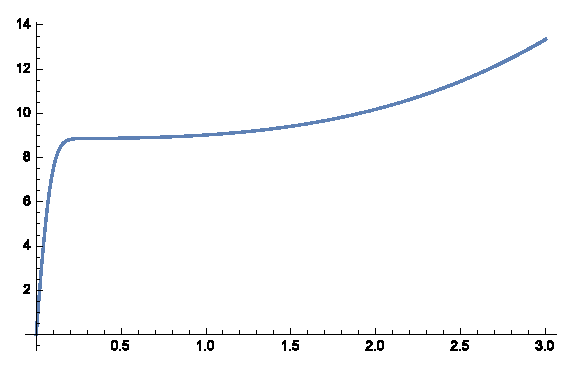
\includegraphics[width=3in]{test1no2}
\caption{Plot of $u(t;\e)$ with $\e=.01$.}
\end{figure}
This suspicion is confirmed when we look at $a(t)=2t$, the coefficient on the first derivative term. Since $a(t)>0$ for $t>0,$ we know there is a layer at $t=0.$
We can then begin to find an outer solution by letting $u(t;\e)\sim u_0(t)$ and collecting only the $O(1)$ terms:
$$2t u_0'=t^3\implies u_0=\frac{t^3}{6}+C.$$
Note we do not apply the initial conditions here. To find the inner solution, then we let $\delta\tau =t,$ and $u(t;\e)=U(\tau;\e).$ We then get
$$\frac{\e}{\delta^2}U''+2\tau U'=\delta^3\tau^3,\quad  U(0)=0,\quad U'(0)=\frac{1}{\sqrt{\e}} .$$
For $\tau=O(1),$ we must balance between the first two terms, giving
$$\frac{\e}{\delta^2}=1\implies \delta=\sqrt{\e}.$$
The differential equation then becomes
$$U''+2\tau U'=\e^{3/2}\tau^3\quad  U(0)=0,\quad U'(0)=\frac{1}{\sqrt{\e}}.$$
We then find the leading order inner solution by letting $U(\tau;\e)\sim U_0(\tau)$ and collecting the $O(1)$ terms. This gives the differential equation
$$U_0''+2\tau U_0'=0,\quad U_0(0)=0,\quad U_0'(0)=\frac{1}{\sqrt{\e}}.$$
This equation has the solution
$$U=\frac{1}{\sqrt{\e}}\int_0^\tau e^{-s^2}ds=\frac{\sqrt{\pi}}{2\sqrt{\e}}erf(\tau).$$
We know match the inner and outer solutions using the Van Dyke matching principle. We express $u_0$ in terms of $\tau$ and $U_0$ in terms of $t$. We get
$$u_0(\tau)=\frac{\e^{3/2}\tau^3}{6}+C,$$
$$U_0=\frac{\sqrt{\pi}}{2\sqrt{\e}}erf\left(\frac{t}{\sqrt{\e}}\right).$$
We then let $\e\to 0$ to find
$$u_0\sim C,\text{ and }U_0\sim\frac{\sqrt{\pi}}{2\sqrt{\e}}\implies C=\frac{\sqrt{\pi}}{2\sqrt{\e}}.$$
Then the composite solution is
$$u_c=\frac{t^3}{6}+\frac{\sqrt{\pi}}{2\sqrt{\e}}erf\left(\frac{t}{\sqrt{\e}}\right).$$
Looking back to the exact solution, we can see that our asymptotic solution is included in the exact solution. Similarly, plotting our asymptotic expansion (located on the top of the next page) shows that the asymptotic and exact solutions are almost entirely equivalent for small $\e.$
\begin{figure}[h]
\centering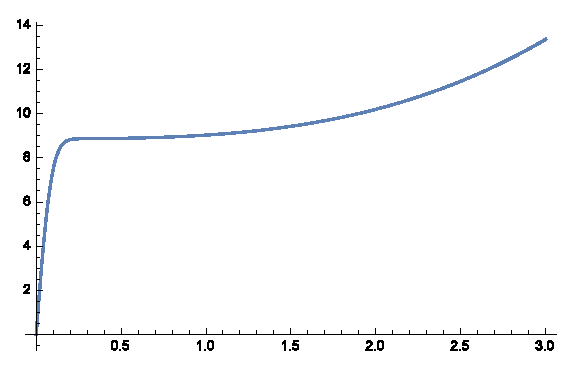
\includegraphics[width=3in]{test1no2prt2}
\caption{Plot of $u_c$ with $\e=.01$.}
\end{figure}
In fact, overlaying them gives no discernable difference whatsoever.
\pagebreak
\item Consider the problem
$$(1+\e)x^2y'=\e[(1-\e)xy^2-(1+\e)x+y^3+2\e y^2],\quad y(1)=1,\quad 0\leq x\leq 1.$$
\benum
\item Compute three terms of an outer expansion.
\item Deduce the location and width of the inner region.
\item Compute two terms of an inner expansion.
\item Form a composite expansion.
\eenum
Solution:\\

\benum
\item We have no reason to believe that the inner region lies at $x=1$ as no singularities occur and no terms are lost in the differential equation here. However, at $x=0$ we lose almost every term, implying that we may have a layer there. Based on the form of the equation, we should expect the outer solution to take the form
$$y(x;\e)\sim y_0(x)+\e y_1(x)+\e^2 y_2(x).$$
Thus we substitute this expression into the equation and collect all terms up to $O(\e^2)$, giving us the new equation:
$$x^2(1+\e)(y_0'+\e y_1')+x^2\e^2 y_2'=-\e x+\e xy_0^2+\e y_0^3-x\e^2+2\e^2y_0^2-\e^2 xy_0^2+2\e^2 x y_0y_1+3\e^2y_0^2y_1,$$
with boundary conditions
$$y_0(1)=1,\quad y_1(1)=0,\quad y_2(1)=0.$$
Then we look at the coefficients of common powers of $\e$ and solve:
$$\e^0:\quad x^2 y_0'=0\implies y_0=1.$$
$$\e^1:\quad x^2y_1'=1\implies y_1=1-\frac{1}{x}.$$
$$\e^2:\quad 1+x^2 y_2'=2-2x+2x(1-\frac{1}{x})+3(1-\frac{1}{x})\implies y_2=-\frac{2}{x}+\frac{3}{2x^2}+\frac{1}{2}.$$
Hence the outer solution is
$$y(x;\e)\sim 1+\e\left(1-\frac{1}{x}\right)+\e^2\left(-\frac{2}{x}+\frac{3}{2x^2}+\frac{1}{2}\right).$$


\item We see that the outer solution contains singularities at $x=0$, implying there is an inner region at $x=0.$ Similarly, the outer solution becomes disordered when $x=O(\e)$ , i.e., if $x=\e$ the outer solution becomes
    $$y(x;\e)\sim 1+\e-1+\frac{3}{2}-2\e+\frac{\e^2}{2}.$$
    Thus we have a layer at $x=0$ of thickness $\e.$ 
    Plotting the outer solution with $\e=.01$ further confirms this.
    \begin{figure}[h]
    \centering
    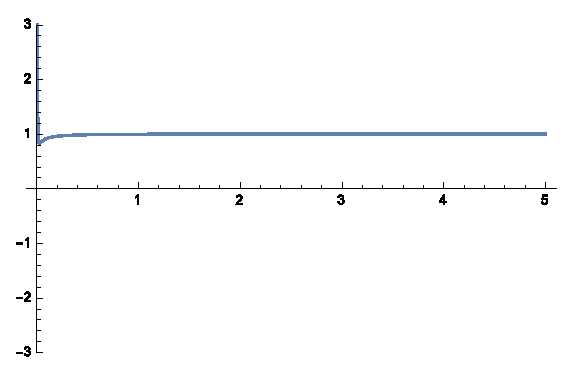
\includegraphics[width=3in]{test1no3prtb}
    \caption{Plot of outer solution with $\e=.01$.}
    \end{figure}

\item To determine the inner solution, we let $x=\e\xi$, and $y(x;\e)=Y(\xi;\e).$ Substituting this into the differential equation allows us to remove the $\e$ in front of the right hand side to give the equation
    $$(1+\e)\xi^2 Y'=[(1-\e)\e\xi Y^2-(1+\e)\e\xi+Y^3+2\e Y^2].$$
    Note that we do not have any boundary conditions for this equation. To determine the leading order inner solution we let $Y(\xi;\e)\sim Y_0(\xi)$ and collect the $O(1)$ terms. We then solve
    $$\xi^2 Y_0'=Y_0^3.$$
    This equation has the solution
    $$Y_0=\pm\sqrt{\frac{\xi}{2-2C\xi}}.$$
    We then match to $O(1)$ of the outer solution:
    $$y(x;\e)\sim 1-\frac{1}{\xi}+\frac{3}{2\xi^2}\text{ as }\e\to 0,$$
    $$Y(\xi;\e)\sim \pm\sqrt{\frac{1}{-2C}}\text{ as }\e\to 0.$$
    Thus we either choose 
    $$C=-\frac{2\xi^4}{(3-2\xi+2\xi^2)^2}\text{ or }C=-\frac{1}{2}.$$
    The second choice makes much more sense, since we are only interested in matching $y_0$ with $Y_0.$ Further, this matching shows that we want only the positive solution of $Y_0.$  Thus we have
    $$Y_0=\sqrt{\frac{\xi}{2+\xi}}.$$
    Now we compute the second term of the inner expansion by letting $Y(\xi;\e)\sim Y_0+\e Y_1.$ When we collect only the $O(\e)$ terms we have
    $$Y_1'-\frac{3}{x(2+x)}Y_1=-\frac{1}{\sqrt{x}(2+x)^{3/2}}.$$
    This equation has solution
    $$Y_1=\frac{\sqrt{\xi}}{(2+\xi)^{3/2}}+D\left(\frac{\xi}{2+\xi}\right)^{3/2}.$$
    Giving us 
    $$Y\sim \sqrt{\frac{\xi}{2+\xi}}+\e\left(\frac{\sqrt{\xi}}{(2+\xi)^{3/2}}+D\left(\frac{\xi}{2+\xi}\right)^{3/2}\right).$$
    We then match with our expansion for the outer solution $y$ to find $D$.
    $$y_0(\xi)+\e y_1(\xi)\sim 1+\e-\frac{1}{\xi},$$
    $$Y_0\to 1+\e D\text{ as }\xi\to \infty, \implies D=1.$$
    Then the inner solution is
    $$Y(\xi;\e)\sim \sqrt{\frac{\xi}{2+\xi}}+\e\frac{\sqrt{\xi}(1+\xi)}{(2+\xi)^{3/2}}$$
    $$Y(x;\e)\sim \sqrt{\frac{x}{2\e+x}}+\e\frac{\sqrt{x}(\e+x)}{(2\e+x)^{3/2}}.$$
    This solution looks like
    \begin{figure}[h]
    \centering
    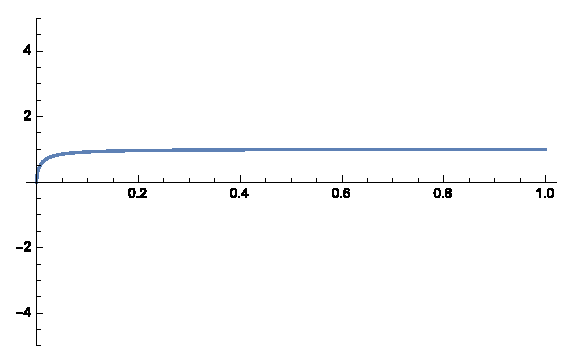
\includegraphics[width=3in]{test1no3prtc}
    \caption{Plot of $Y_0(x)+\e Y_1(x)$ with $\e=.01$.}
    \end{figure}

\item The composite solution in this case is quite different from previous composites we have looked at. On one hand, we are doing basically the same thing in adding the outer and inner solutions then subtracting their common parts, but we must remove the singularities present in the outer solution. We can do this in two ways. We can choose to create a piecewise-continuous composite solution of the form
    $$y_c(x;\e)=\left\{\begin{array}{cc}y_0(x)+\e y_1(x)+\e^2 y_2(x),&\e<x\leq1\\ \\Y_0(x)+\e Y_1(x),&0\leq x\leq a\end{array}\right.=\left\{\begin{array}{cc}1+\e\left(1-\frac{1}{x}\right)+\e^2\left(-\frac{2}{x}+\frac{3}{2x^2}+\frac{1}{2}\right),&\e<x\leq 1\\ \\ \sqrt{\frac{x}{2\e+x}}+\e\frac{\sqrt{x}(\e+x)}{(2\e+x)^{3/2}},&0\leq x\leq a\end{array}\right..$$
    Graphing this, with $a=10\e$ and $\e=.01$, gives the solution:
    \begin{figure}[h]
    \centering
    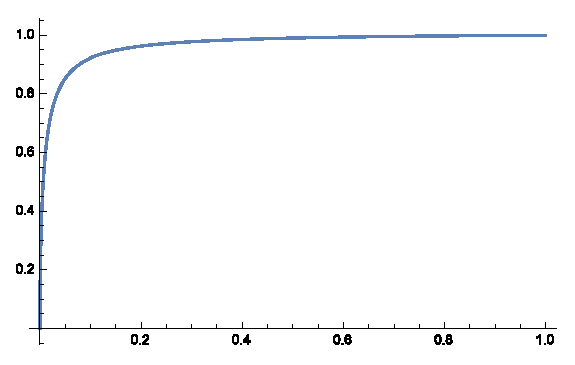
\includegraphics[width=3in]{test1no3prtd1}
    \caption{Plot of Piecewise composite solution}
    \end{figure}
    Or we can choose to simply add together the inner and outer solutions, remove their common parts, and remove the terms that cause singularities.
    $$y_c(x;\e)=y_0(x)+\e y_1(x)+\e^2 y_2(x)+ Y_0(x)+\e Y_1(x)-1-\e-\text{singularities},$$
    $$y_c(x;\e)=\sqrt{\frac{x}{2\e+x}}+\e\frac{\sqrt{x}(\e+x)}{(2\e+x)^{3/2}}+\frac{\e^2}{2}.$$
    This solution looks like
    \begin{figure}[h]
    \centering
    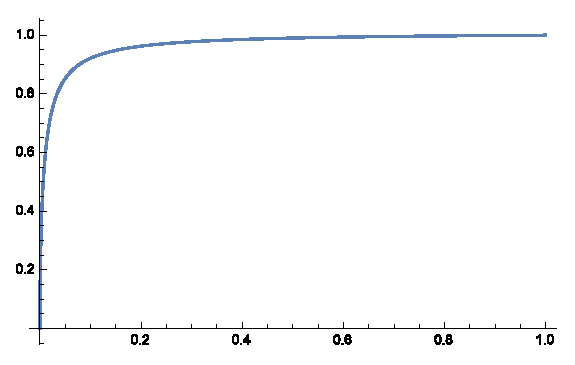
\includegraphics[width=3in]{test1no3prtd2}
    \caption{Plot of continuous composite solution}
    \end{figure}
    As we can see, both solutions remove the singularity at $x=0$ and have the proper shape. They are nearly indistinguishable from one another.

\eenum
\eenum
\end{document}